% context: markscheme (official solutions) for 2-9HW_Kinematics-review
% topic: a one-chain conversion, a two-step rate problem, displacement and average
%        velocity, braking from a stopping distance, a velocity-time graph with a
%        braking segment, a ball thrown up, a height-time parabola and its velocity
%        graph
% convention: answers in bold; "=" joins exact equalities, "\approx" introduces a
%        rounded value; each problem names the skill it practises
\documentclass[12pt, twoside]{article}
%\documentclass[12pt, twoside]{article}
\usepackage[letterpaper, margin=1in, headsep=0.2in]{geometry}
\setlength{\headheight}{0.6in}
%\usepackage[english]{babel}
\usepackage[utf8]{inputenc}
\usepackage{microtype}
\usepackage{amsmath}
\usepackage{amssymb}
%\usepackage{amsfonts}
\usepackage[nomessages]{fp} %\FPeval{\var-name}{2*sin(pi/6)}
\usepackage{siunitx} %units in math. eg 20\milli\meter
\usepackage{yhmath} % for arcs, overparenth command
\usepackage{tikz} %graphics
\usetikzlibrary{quotes, angles, arrows, arrows.meta}
\usepackage{graphicx} %consider setting \graphicspath{{images/}}
\usepackage{parskip} %no paragraph indent
\usepackage{enumitem}
\usepackage{multicol}
\usepackage{venndiagram}

\usepackage{fancyhdr}
\pagestyle{fancy}
\fancyhf{}
\renewcommand{\headrulewidth}{0pt} % disable the underline of the header
\raggedbottom
\hfuzz=2mm %suppresses overfull box warnings

\usepackage{hyperref}
\usepackage{float}
\setlength{\parskip}{0.2\baselineskip}
\sisetup{reset-text-series=false, reset-math-version=false, text-series-to-math=true}

\title{Physics}
\author{Chris Huson}
\date{November 2026}

\fancyhead[LE]{\thepage}
\fancyhead[RO]{\thepage}
\fancyhead[LO]{La Scuola d'Italia / Huson / Physics \\* 13 November 2026}

\begin{document}

\subsubsection*{2.9 Homework: Kinematics Review Solutions}

\begin{enumerate}[itemsep=0.5cm]

\item \emph{Skill: unit conversion.} One chain, evaluated once:

  $72\,\dfrac{\text{floors}}{\text{min}} \times \dfrac{4.0~\text{m}}{1~\text{floor}}
  \times \dfrac{1~\text{min}}{60~\text{s}} = \mathbf{4.8~\textbf{m/s}}$

  \emph{Exact, so no rounding. ``Floors'' cancels like any other unit. Sense check:
  4.8 m/s is about 17 km/h, a fast bicycle. The usual error is
  $\frac{60~\text{s}}{1~\text{min}}$ upside down, giving 17\,280.}

\item \emph{Skill: rate problem.} Knowns: $v = 5.83$ m/s, $d = 42.195$ km
  $= \num{42195}$ m.

  Step 1, the rate relationship: \quad $t = \dfrac{d}{v} =
  \dfrac{\num{42195}~\text{m}}{5.83~\text{m/s}} = 7237.56\ldots~\text{s}$

  Step 2, convert, carrying the unrounded value: \quad
  $7237.56\ldots~\text{s} \times \dfrac{1~\text{h}}{3600~\text{s}} = 2.0104\ldots
  \approx \mathbf{2.01~\textbf{h}}$

  \emph{Three figures, from 5.83. That is just over two hours (about 2 h 0 min 38 s).
  Do not write 2.01 h as ``2 h 1 min'': 0.01 h is 0.6 min.}

\newpage

\item \emph{Skill: distance and displacement, speed and velocity.} Arrows: $-15$ m
  from 0 to $-15$, then $+6$ m from $-15$ to $-9$.
  \begin{enumerate}[itemsep=0.3cm]
    \item $x = -15 + 6 = \mathbf{-9~\textbf{m}}$, that is, 9 m west of the door.
    \item Distance $= 15 + 6 = \mathbf{21~\textbf{m}}$ \qquad Displacement
      $= \mathbf{-9~\textbf{m}}$ (9 m west)
    \item Total time $= 10.0 + 5.0 = 15.0$ s.

      average speed $= \dfrac{21~\text{m}}{15.0~\text{s}} = \mathbf{1.4~\textbf{m/s}}$
      \qquad
      $\bar{v} = \dfrac{-9~\text{m}}{15.0~\text{s}} = \mathbf{-0.60~\textbf{m/s}}$,
      that is, 0.60 m/s west

      \emph{Credit $\bar{v}$ only with its sign or direction.}
  \end{enumerate}

\item \emph{Skill: constant-acceleration equations.} Knowns: $v_0 = 31.3$ m/s,
  $v = 0$, $x - x_0 = 75$ m.
  \begin{enumerate}[itemsep=0.3cm]
    \item No time is given, so use $v^2 = v_0^2 + 2a(x - x_0)$:

      $a = \dfrac{v^2 - v_0^2}{2(x - x_0)} = \dfrac{0 - 31.3^2}{2 \times 75~\text{m}}
      = \dfrac{-979.69}{150} = -6.531\ldots \approx
      \mathbf{-6.5~\textbf{m/s}^\mathbf{2}}$

      \emph{Two figures, from 75 m. Negative, because the car slows while moving in
      the positive direction.}
    \item $\bar{v} = \dfrac{v + v_0}{2} = \dfrac{0 + 31.3}{2} = 15.65$ m/s, so
      $t = \dfrac{x - x_0}{\bar{v}} = \dfrac{75~\text{m}}{15.65~\text{m/s}} =
      4.79\ldots \approx \mathbf{4.8~\textbf{s}}$

      \emph{Also accept $t = \frac{v - v_0}{a} = \frac{0 - 31.3}{-6.531\ldots} =
      4.79$ s, using the unrounded $a$. With $a = -6.5$ the answer is still 4.8 s.}
  \end{enumerate}

\newpage

\item \emph{Skill: motion graphs.}

  \begin{center}
  \begin{tikzpicture}[x=0.92cm, y=0.42cm]
    \draw[gray!25, thin, xstep=0.5, ystep=1] (0,0) grid (14,12);
    \draw[gray!60, xstep=1, ystep=2] (0,0) grid (14,12);
    \draw[->, thick] (0,0) -- (14.5,0) node[right]{\small $t$ (s)};
    \draw[->, thick] (0,0) -- (0,13) node[above]{\small $v$ (m/s)};
    \foreach \t in {0,...,14} \node[below] at (\t,0) {\scriptsize \t};
    \foreach \v in {2,4,...,12} \node[left] at (0,\v) {\scriptsize \v};
    \draw[very thick] (0,0) -- (5,10) -- (9,10) -- (13,0);
    \draw[dashed] (3,0) -- (3,6) -- (0,6);
    \fill (3,6) circle (2.5pt);
  \end{tikzpicture}
  \end{center}

  \begin{enumerate}[itemsep=0.3cm]
    \item \textbf{6 m/s}, read from the line at $t = 3.0$ s.
    \item slope $= \dfrac{10 - 0~\text{m/s}}{5.0 - 0~\text{s}} =
      \mathbf{2.0~\textbf{m/s}^\mathbf{2}}$
    \item \textbf{Zero}: the line is flat. \textbf{The bus moves at a constant
      10 m/s.}

      \emph{Not ``the bus has stopped''. It stops only where $v = 0$, at 13 s.}
    \item slope $= \dfrac{0 - 10~\text{m/s}}{13.0 - 9.0~\text{s}} =
      \mathbf{-2.5~\textbf{m/s}^\mathbf{2}}$. \textbf{The bus is slowing down}: the
      acceleration is opposite to the velocity, which is still positive.
  \end{enumerate}

\item \emph{Skill: free fall.} Up positive: $v_0 = +24.5$ m/s, $a = -9.80$ m/s$^2$.
  \begin{enumerate}[itemsep=0.3cm]
    \item \textbf{Velocity $\mathbf{v = 0}$}, for an instant. \textbf{Acceleration
      $\mathbf{a = -9.80}$ m/s$^\mathbf{2}$}, the same as during the rest of the
      flight.

      \emph{The common wrong answer is $a = 0$ at the top.}
    \item $t = \dfrac{v - v_0}{a} = \dfrac{0 - 24.5~\text{m/s}}{-9.80~\text{m/s}^2}
      = \mathbf{2.50~\textbf{s}}$
    \item $\bar{v} = \dfrac{0 + 24.5}{2} = 12.25$ m/s, so
      $y - y_0 = \bar{v}\,t = 12.25~\text{m/s} \times 2.50~\text{s} = 30.625
      \approx \mathbf{30.6~\textbf{m}}$

      \emph{Also accept $y - y_0 = \frac{0 - 24.5^2}{2(-9.80)} = 30.6$ m. About ten
      storeys.}
  \end{enumerate}

\newpage

\item \emph{Skill: motion graphs (free fall).} Here $y = 12t - 5t^2$ and
  $v = 12 - 10t$.

  \begin{tikzpicture}[x=2.3cm, y=0.42cm]
    \draw[gray!25, thin, xstep=0.1, ystep=0.5] (0,0) grid (2.4,8);
    \draw[gray!60, xstep=0.4, ystep=2] (0,0) grid (2.4,8);
    \draw[->, thick] (0,0) -- (2.52,0) node[below right]{\small $t$ (s)};
    \draw[->, thick] (0,0) -- (0,8.8) node[above]{\small $y$ (m)};
    \foreach \t in {0,0.4,0.8,1.2,1.6,2.0,2.4} \node[below] at (\t,0) {\scriptsize \t};
    \foreach \y in {2,4,6,8} \node[left] at (0,\y) {\scriptsize \y};
    \draw[very thick, domain=0:2.4, samples=60] plot (\x, {12*\x - 5*\x*\x});
    \draw[thick, dashed] (0,0) -- (1.2,7.2);
    \draw[thick] (0.8,7.2) -- (1.6,7.2);
  \end{tikzpicture}
  \hfill
  \begin{tikzpicture}[x=2.3cm, y=0.14cm]
    \draw[gray!25, thin, xstep=0.1, ystep=1] (0,-12) grid (2.4,12);
    \draw[gray!60, xstep=0.4, ystep=4] (0,-12) grid (2.4,12);
    \draw[->, thick] (0,0) -- (2.52,0) node[above right]{\small $t$ (s)};
    \draw[->, thick] (0,-12) -- (0,13.5) node[above]{\small $v$ (m/s)};
    \foreach \t in {0.4,0.8,1.2,1.6,2.0,2.4}
      \node[below, fill=white, inner sep=1pt] at (\t,-0.4) {\scriptsize \t};
    \foreach \v in {-12,-8,...,12} \node[left] at (0,\v) {\scriptsize \v};
    \draw[very thick] (0,12) -- (2.4,-12);
  \end{tikzpicture}

  \begin{enumerate}[itemsep=0.3cm]
    \item Highest at $\mathbf{t = 1.2~\textbf{s}}$, \textbf{7.2 m} up.

      \emph{Check: $12(1.2) - 5(1.2)^2 = 14.4 - 7.2 = 7.2$ m. Accept readings
      within one small square.}
    \item \textbf{Zero}: the tangent at the top is flat (solid line). So
      $\mathbf{v = 0}$ there.
    \item Chord (dashed): slope $= \dfrac{7.2 - 0~\text{m}}{1.2 - 0~\text{s}} =
      \mathbf{6.0~\textbf{m/s}}$. \textbf{It is the average velocity on the way up.}

      \emph{It is half of 12 m/s, as $\bar{v} = \frac{v + v_0}{2} = \frac{0 + 12}{2}$
      predicts.}
    \item A straight line from $+12$ m/s at $t = 0$ down to $-12$ m/s at
      $t = 2.4$ s. It crosses zero at \textbf{1.2 s}, the top. It lands at
      $\mathbf{-12~\textbf{m/s}}$: the same speed it was kicked at, now downward.
  \end{enumerate}

\end{enumerate}
\end{document}
